\documentclass[12pt]{article}
\usepackage[utf8]{inputenc}
\usepackage{array}
\newcolumntype{C}[1]{>{\centering\let\newline\\\arraybackslash\hspace{0pt}}m{#1}}
\usepackage[spanish]{babel}
 \usepackage{url}
\usepackage[spanish, fixlanguage]{babelbib}
\bibliographystyle{IEEEtran}
\usepackage{graphicx}
\graphicspath{ {./images/} }
\usepackage{amssymb}
\usepackage{amsmath}
\usepackage{subcaption}
\usepackage[linesnumbered]{algorithm2e}
\usepackage{tikz}
\usetikzlibrary{positioning, fit}
\usetikzlibrary{babel}

\title{Tarea 4}

\author{
	Saul Ivan Rivas Vega \\
	\\
	Diseño y análisis de algoritmos\\
\\
	Equipo Completo:\\
		Yadira Fleitas Toranzo\\
		Diego de Jesús Isla Lopez\\
		Saul Ivan Rivas Vega\\
}

\date{\today}

\begin{document}
	\maketitle
	\pagebreak
	\section{Ejercicio 1.}
	\subsection{Da un ejemplo de una familia de digráficas de $n$ vértices con pesos no negativos tal que admita una ejecución del algoritmo de Dijkstra en la cual todos los nodos actualizan a su padre y su estimación de distancia $d(v)$ una sola vez; es decir, la primera oferta de camino que reciben, es la del camino mas corto. Demuestra que tu ejemplo cumple lo que se pide.}
	\paragraph{}Sea $F$ la familia de digráficas que cumpla las siguientes condiciones para cada miembro $G$ de ella:\\
	\begin{itemize}
		\item La gráfica $G$ tiene un conjunto de aristas ponderadas $E$ tal que $|E| = n$ donde cada arista tiene un peso mayor o igual a cero y un conjunto de vértices $V$ tal que $|V| = n$.
		\item $G$ es conexa.
		\item Todo $v\in V$ tiene $inDegree(v) = 1$, es decir que tienen exactamente una sola arista de entrada.
		\item Todo $v\in V$ tiene $outDegree(v) = 1$, es decir que tienen exactamente una sola arista de salida. 
		\item Solo hay un ciclo y todo $v\in V$ esta en el ciclo.
	\end{itemize}
	Un miembro de esta familia con $n=6$ es:\\
	\begin{center}
	\begin{tikzpicture}[roundnode/.style={draw,shape=circle,fill=black!40,minimum size=1mm}]
		\tikz
		%Nodes
		\node[roundnode,label={north west:$v_1$}]      (v1)                     {};
		\node[roundnode,label={north east:$v_2$}]      (v2)       [right=of v1] {};
		\node[roundnode,label={east:$v_3$}]      (v3)       [below right=of v2] {};
		\node[roundnode,label={south east:$v_4$}]      (v4)       [below left =of v3] {};
		\node[roundnode,label={south west:$v_5$}]      (v5)       [left =of v4] {};
		\node[roundnode, label={west:$v_6$}]      (v6)       [below left =of v1] {};
		%Lines
		\draw[->] (v1) -- (v2) node[midway,below] {2};
		\draw[->] (v2) -- (v3) node[midway,below] {4};
		\draw[->] (v3) -- (v4) node[midway,below] {1};
		\draw[->] (v4) -- (v5) node[midway,below] {4};
		\draw[->] (v5) -- (v6) node[midway,below] {0};
		\draw[->] (v6) -- (v1) node[midway,below] {5}; 
	\end{tikzpicture}
	\end{center}
	\paragraph{Demostración} Por contradicción.\\
	Supongamos que durante una ejecución el algoritmo de Dijkstra al empezar en cualquier nodo $s\in G$, existe un nodo $v_i$ tal que $v_i \neq s$ y además actualizó su estimación de distancia $d(v_i)$ mas de una vez.\\
	Entonces el algoritmo hizo una primera estimación de distancia $d(v_i)_1$ siguiendo un camino de nodos $p$ desde $s$ hasta $v_i$. Ahora para realizar una estimación adicional $d(v_i)_2$ tal que $d(v_i)_2 < d(v_i)_1$ debió encontrar un segundo camino $p'$ para llegar a $v_i$.\\
	Sin embargo, siendo $G$  miembro de la familia $F$ se cumple que todo $v\in G$ tiene una sola arista de salida y una de entrada, y solo hay un ciclo donde todo $v\in G$ esta en el. Le sigue que, para llegar a $v_i$ desde $s$, se puede:
	\begin{enumerate}
		\item Seguir el ciclo hasta llegar a $v_i$.
		\item Completar el ciclo $z$ veces ($z>=1$) y volver a llegar a $v_i$.
	\end{enumerate}  
	El camino resultante de al usar el segundo método será siempre mayor o igual al primero puesto que los pesos son mayores o iguales a 0 manteniendo o incrementando el camino del primer método.\\
	Por lo tanto existe un solo camino mínimo entre cualquier par de nodos en $G$. Entonces no existe un segundo camino $p'$ tal que al llegar a $v_i$ su estimación de distancia cumpla que $d(v_i)_2 < d(v_i)_1$ y en la ejecución no hubo una actualización adicional a la primera, pero esto es una contradicción a nuestra suposición inicial. Finalmente, en cualquier ejecución del algoritmo empezando en cualquier nodo $s\in G$, todos los nodos actualizan a su padre y su estimación de distancia $d(v_i)$ una sola vez.
	\pagebreak
	\subsection{Da un ejemplo de una familia de digráficas con pesos no negativos tal que cualquier ejecución del algoritmo de Dijkstra requiera que algún vértice actualice su padre y su estimación de distancia dos veces. Demuestra que tu ejemplo cumple lo que se pide.}
		\paragraph{}Sea $F$ la familia de digráficas que cumpla las siguientes condiciones para cada miembro $G$ de ella:\\
	\begin{enumerate}
		\item Tiene un nodo inicial $s$ el cual no tiene aristas de entrada.
		\item $s$ tiene una arista de salida con peso igual a 1.
		\item Tiene un nodo final $v_f$ el cual no tiene aristas de salida.
    	\item $v_f$ tiene una arista de entrada con peso igual a 1.
		\item Para todo $v\in G$ tal que $v\neq s$ y $v\neq v_f$, se cumple:
			\begin{enumerate}
				\item $v$ tiene una sola arista de entrada con peso igual a 1.
				\item $v$ tiene una sola arista de salida con peso igual a 1.
			\end{enumerate}
	\item Desde $s$ se puede llegar a todos los otros vértices.
	\item Hay una arista adicional desde $s$ a $v_f$ con peso $2n$.
	\item $s$ tiene exactamente 2 aristas de salida.
	\item $v_f$ tiene exactamente 2 aristas de entrada.
	\end{enumerate}
	Un miembro de esta familia con $n=4$, donde $s = v_1$ y $v_f = v_4$ es:\\
	\begin{center}
		\begin{tikzpicture}[roundnode/.style={draw,shape=circle,fill=black!40,minimum size=1mm}]
		\tikz
		%Nodes
		\node[roundnode,label={north west:$v_1$}]      (v1)                     {};
		\node[roundnode,label={north west:$v_2$}]      (v2)       [right=of v1] {};
		\node[roundnode,label={north west:$v_3$}]      (v3)       [right=of v2] {};
		\node[roundnode,label={north west:$v_4$}]      (v4)       [right =of v3] {};
		%Lines
		\draw[->] (v1) -- (v2) node[midway,below] {1};
		\draw[->] (v2) -- (v3) node[midway,below] {1};
		\draw[->] (v3) -- (v4) node[midway,below] {1};
		\draw[->] (v1) to [out=270,in=240] node[pos=0.5, below] {8}  (v4) ;
		\end{tikzpicture}
	\end{center}
	\paragraph{Demostración} Propongamos al vértice $v_f$ como aquel nodo que actualice su padre y su estimación de distancia dos veces al comenzar desde el nodo $s$.\\
	La primer estimación de distancia $d(v_f)_1$se realiza al ejecutar el algoritmo iniciando en $s$, pues $v_f$ es vecino directo por la propiedad $7$. $d(v_f)_1$ vale $2n$. Ahora para una segunda estimación se puede seguir el camino de la otra arista de peso 1 de  $s$, dicho camino llegará a $v_f$ por  la propiedad $6$. \\ Este camino tendrá como peso total la suma de los pesos de las aristas, cada arista en ese camino tiene peso 1, y como pasa por todos los nodos y todos menos $v_f$ tienen una arista de salida de peso 1, significa que hay $n-1$ aristas. Posteriormente tenemos que esta segunda estimación $d(v_f)_2$ vale $n-1$. Finalmente como $d(v_f)_2  < d(v_f)_1$ habrá forzosamente una segunda actualización.
	\section{Ejercicio 2.}
	\subsection{De acuerdo con el algoritmo de Dijkstra que revisamos en clase, para cada $n\in \mathbb{N}$ con $n>2$, presenta una familia de gráficas de $n$ vértices con pesos tanto positivos como negativos y sin ciclos dirigidos de longitud negativa para la cual se cumple que si $G$ es una gráfica de la familia, el algoritmo de Dijkstra falla en encontrar el camino más corto entre $s$ y algún otro vértice de $G$. Demuestra que de hecho existe tal vértice.}
	\paragraph{}Sea $F$ la familia de digráficas que sigue el siguiente proceso de construcción:\\
	Para $G_0$ se tiene la siguiente gráfica:
		\begin{center}
			\begin{tikzpicture}[roundnode/.style={draw,shape=circle,fill=black!40,minimum size=1mm}]
			\tikz
			%Nodes
			\node[roundnode,label={north west:$v_1$}]      (v1)                     {};
			\node[roundnode,label={north west:$v_2$}]      (v2)       [above right=of v1] {};
			\node[roundnode,label={north east:$v_3$}]      (v3)       [below right=of v2] {};
			%Lines
			\draw[->] (v1) -- (v2) node[midway,above] {$z$};
			\draw[->] (v2) -- (v3) node[midway,above] {$-z$};
			\draw[->] (v1) -- (v3) node[midway,below] {1};
			\end{tikzpicture}
		\end{center}
		Donde $z = 2n$, en $G_0$ $z=6$.\\
		Ahora para cualquier otro $G_i$ con $i>0$ se agregará una arista del último nodo de $G_{i-1}$, el cual es $v_{i+2}$, a un nuevo nodo $v_{i + 3}$ con peso 1: 
				\begin{center}
			\begin{tikzpicture}[roundnode/.style={draw,shape=circle,fill=black!40,minimum size=1mm}]
			\tikz
			%Nodes
			\node[roundnode,label={north west:$v_1$}]      (v1)                     {};
			\node[roundnode,label={north west:$v_2$}]      (v2)       [above right=of v1] {};
			\node[roundnode,label={north east:$v_3$}]      (v3)       [below right=of v2] {};
			\node[label={$...$}]      (v4)       [right=of v3] {};
			\node[roundnode,label={north east:$v_{i+2}$}]      (v5)       [right=of v4] {};
    		\node[roundnode,label={north east:$v_{i+3}$}]      (v6)       [right=of v5] {};
			%Lines
			\draw[->] (v1) -- (v2) node[midway,above] {$z$};
			\draw[->] (v2) -- (v3) node[midway,above] {$-z$};
			\draw[->] (v1) -- (v3) node[midway,below] {1};
			\draw[->] (v3) -- (v4) node[midway,below] {1};
			\draw[->] (v4) -- (v5) node[midway,below] {1};
    		\draw[->] (v5) -- (v6) node[midway,below] {1};
			\end{tikzpicture}
		\end{center}
	\paragraph{Demostración} La ejecución de Dijkstra empieza en $v_1$ y propongamos que donde falla en encontrar el camino mínimo es para el nodo $v_3$.\\
	En la primera ocasión donde se estiman distancias a partir de $v_1$ se marca como explorados a $v_2$ y a $v_3$.
	La estimaciones son: $d(v_2)=z$ y $d(v_3)=1$. Esas son las primeras estimaciones para cualquier ejecución del algoritmo con nodo inicial en $v_1$.\\
	Ahora como $z=2n$ y $2n>1$ el algoritmo seguirá explorando ahora con $v_3$. Solo se consideraría ir por $v_2$ cuando la estimación de distancia para algún nodo $v_i$ cumpla que $d(v_i) > 2n$, sin embargo como las aristas tienen peso 1, y no hay mas de $n-3$ aristas a partir de $v_3$, nunca se considerará explorar a partir de $v_2$.\\
	Por lo tanto al explorar todos los nodos se terminará la ejecución del algoritmo y la estimación de distancia para $v_3$ es $d(v_3)=1$, sin embargo al tomar el camino de $v_1$ a $v_2$ y luego a $v_3$ se tendría una distancia de $0$, la cual es menor a $1$. Finalmente para cualquier gráfica $G$ miembro de la familia al ejecutar el algoritmo de Dijkstra empezando en $v_1$, el algoritmo fallará en encontrar la distancia mínima para el nodo $v_3$.
	\subsection{Toma una gráfica de la familia que propones y muestra que Bellman-Ford si encuentra el camino que Dijkstra no.}
	Tomemos a $G_0$:
	\begin{center}
		\begin{tikzpicture}[roundnode/.style={draw,shape=circle,fill=black!40,minimum size=1mm}]
		\tikz
		%Nodes
		\node[roundnode,label={north west:$v_1$}]      (v1)                     {};
		\node[roundnode,label={north west:$v_2$}]      (v2)       [above right=of v1] {};
		\node[roundnode,label={north east:$v_3$}]      (v3)       [below right=of v2] {};
		%Lines
		\draw[->] (v1) -- (v2) node[midway,above] {$6$};
		\draw[->] (v2) -- (v3) node[midway,above] {$-6$};
		\draw[->] (v1) -- (v3) node[midway,below] {1};
		\end{tikzpicture}
	\end{center}
	\begin{algorithm}[H]\footnotesize
	\SetAlgoLined
	Inicializar $d(v)=infinito$, para toda $v \in G$\;
	Asignar $d(s)=0$\;
	\For{i desde 1 hasta (n-1)}{
		\ForEach{Arista $(u,v,peso) \in E$}{ 
				\If{$d(u) + peso < d(v)$}{\emph{$d(v) := d(u) + peso$}\;}
		}
	}
	\caption{Bellman-Ford.}
	\end{algorithm}
	\paragraph{Demostración} Sea $v_1$ el nodo $s$ para el algoritmo.\\
	Al inicializar las distancias como en las lineas 1 y 2 tenemos:
	\begin{itemize}
		\item $d(v_1)=0$. 
		\item $d(v_2)=infinito$.
		\item $d(v_3)=infinito$.
	\end{itemize}
	En la primera ejecución del ciclo en la linea 3 se prueban las siguientes aristas con las correspondientes evaluaciones:
	\begin{itemize}
		\item Arista$(v_1, v_2, 6)$.
		\begin{itemize}
				\item $d(v_1) + 6 < d(v_2)$.
				\item $0 + 6 < infinito$.
				\item true. Asignamos $d(v_2) := 6$
			\end{itemize}
	\item La arista $(v_1, v_3, 1)$ pudo haber sido evaluada en dos casos:
	\begin{enumerate}
		\item Cuando $d(v_3)=infinito - 6$, es decir evaluamos primero a la arista $(v_2, v_3, -6)$.
		\begin{itemize}
			\item $d(v_1) + 1 < d(v_3)$.
			\item $1 < infinito-6$.
			\item true. Asignamos $d(v_3) := 1$
		\end{itemize}
		\item Cuando $d(v_3)=infinito$, es decir todavía no evaluamos a la arista $(v_2, v_3, -6)$.
		\begin{itemize}
			\item $d(v_1) + 1 < d(v_3)$.
			\item $0 + 1 < infinito$.
			\item true. Asignamos $d(v_3) := 1$
		\end{itemize}
		
	\end{enumerate}
		\item La arista $(v_2, v_3, -6)$ pudo haber sido evaluada en los mismos dos casos:
		\begin{enumerate}
			 \item Cuando $d(v_2)=infinito$, es decir todavía no evaluamos a la arista $(v_1, v_2, 6)$.
			 \begin{itemize}
			 	\item $d(v_2) + (-6) < d(v_3)$.
			 	\item $infinito - 6 < infinito$.
			 	\item true. Asignamos $d(v_3) := infinito - 6$
			 \end{itemize}
			 \item Cuando $d(v_2)=6$, es decir evaluamos primero a la arista $(v_1, v_2, 6)$.
			 \begin{itemize}
			 	\item $d(v_2) + (-6) < d(v_3)$.
			 	\item $6 - 6 < infinito$.
			 	\item true. Asignamos $d(v_3) := 0$
			 \end{itemize}
		\end{enumerate}
	\end{itemize}
	De haber sido el caso número 2, la distancia ya es correcta para $v_3$ siendo $d(v_3)=0$, sin embargo esa distancia se alcanza en la segunda iteración para el caso número 1:
	\begin{itemize}
	\item La arista $(v_2, v_3, -6)$ tomando el caso numero 1 de la iteración anterior se realiza la siguiente evaluación:
			\begin{itemize}
				\item $d(v_2) + (-6) < d(v_3)$.
				\item $6 - 6 < 1$.
				\item true. Asignamos $d(v) := 0$
			\end{itemize}
	\end{itemize}
Finalmente se asegura que Bellman-Ford llega a la distancia correcta de $v_3$ siendo $d(v_3)=1$, a diferencia de Dijkstra que reportaría erróneamente $d(v_3)=1$ como se muestra en la demostración del ejercicio 2.1.
\section{Ejercicio 3}
\subsection{De acuerdo con el algoritmo de Dijkstra que revisamos en clase, para cada $n\in \mathbb{N}$ con $n>2$, presenta una familia de gráfircas de $n$ vértices con pesos positivos y negativos y sin ciclos dirigidos de longitud negativa para la cual se cumple que si $G$ es una gráfica de la familia, el algoritmo de Dijkstra no falla en encontrar el camino más corto entre dos vértices de $G$. Prueba que en efecto el algoritmo encuentra los caminos más cortos.}
\paragraph{}
	Para $G_0$ se tiene la siguiente gráfica:
\begin{center}
	\begin{tikzpicture}[roundnode/.style={draw,shape=circle,fill=black!40,minimum size=1mm}]
	\tikz
	%Nodes
	\node[roundnode,label={north west:$v_1$}]      (v1)                     {};
	\end{tikzpicture}
\end{center}
Es decir un solo nodo $v_1$. Ahora para cualquier otro $G_i$ con $i>0$ se agregará un nuevo nodo $v_{i+1}$ y una arista de $v_{i} $ a $v_{i+1}$ con peso $w_i$ positivo, negativo o igual a 0. 
\begin{center}
	\begin{tikzpicture}[roundnode/.style={draw,shape=circle,fill=black!40,minimum size=1mm}]
	\tikz
	%Nodes
	\node[roundnode,label={north :$v_1$}]      (v1)                     {};
	\node[roundnode,label={north :$v_2$}]      (v2)       [ right=of v1] {};
	\node[label={$...$}]      (v3)       [right=of v2] {};
	\node[roundnode,label={north :$v_{i}$}]      (v4)       [right=of v3] {};
	\node[roundnode,label={north :$v_{i+1}$}]      (v5)       [right=of v4] {};
	%Lines
	\draw[->] (v1) -- (v2) node[midway,above] {$w_1$};
	\draw[->] (v2) -- (v3) node[midway,above] {$w_2$};
	\draw[->] (v3) -- (v4) node[midway,above] {$w_{i-1}$};
	\draw[->] (v4) -- (v5) node[midway,above] {$w_{i}$};
	\end{tikzpicture}
\end{center}
	\paragraph{Demostración} En este caso cualquier gráfica $G_i$ miembro de la familia tendrá $i$ aristas así como $i+1$ vértices, lo que resulta en que solo exista un camino a seguir estando en cualquier vértice $v\in G_i$. En cualquier ejecución de Dijkstra tomando  cualquier vértice $v$ como vértice inicial $s$, se recorrerá ese único camino que empieza en $s$. Para cualquier vértice en el conjunto de vértices que es posible explorar desde $s$, se encontrará el camino mínimo pues es único y se recorren todos los vértices sin explorar que son alcanzables desde $s$. Finalmente sin importar que se tengan pesos positivos, negativos o iguales a 0, si $G$ es miembro de la familia descrita, el algoritmo de Dijkstra no falla en encontrar el camino más corto entre dos vértices de $G$.
\section{Ejercicio 4. }
\subsection{Considera la estructura de datos de cola de prioridad, implementada con heaps binarios, y el arreglo $A=(10, 12, 1, 14, 6, 5, 8, 15, 3, 9, 7, 4, 11, 13, 2)$. Explica cómo construyes una cola de prioridad que tenga los elementos de A (tienes que dar la construcción del árbol binario); no puedes ordenar el arreglo de entrada antes de crear la cola. Escribe explícitamente la cola resultante.}
\paragraph{} La cola de prioridad se construye agregando cada elemento como la siguiente hoja en el árbol binario, sin embargo en caso que sea menor a su padre cambiará lugar con su padre hasta que su padre no sea mayor o termine siendo la raíz.
\begin{figure}
	\begin{subfigure}{.25\textwidth}
		\centering
		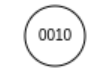
\includegraphics[width=.4\linewidth]{hp001}
		\caption{Elemento inicial 10.}
		\label{fig:sfig1}
	\end{subfigure}
	\begin{subfigure}{.3\textwidth}
		\centering
		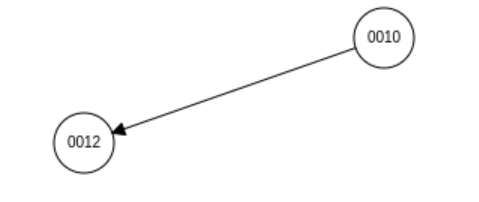
\includegraphics[width=1.4\linewidth]{hp002}
		\caption{Se agrega 12 y como es mayor solo se agrega como hoja.}
		\label{fig:sfig2}
	\end{subfigure}
	\begin{subfigure}{.3\textwidth}
		\centering
		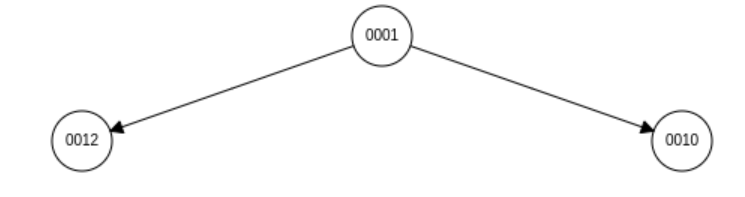
\includegraphics[width=1.8\linewidth]{hp003}
		\caption{1 es menor que todos los elementos así que se agrega como hoja, pero sube hasta la raíz.}
		\label{fig:sfig3}
	\end{subfigure}
	\begin{subfigure}{.6\textwidth}
		\centering
		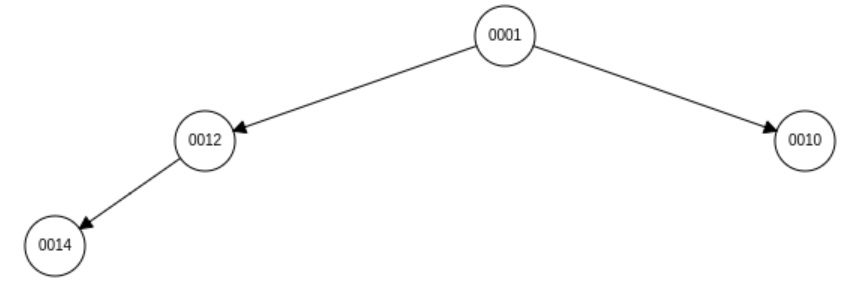
\includegraphics[width=1.04\linewidth]{hp004}
		\caption{14 es mayor que todos los otros elementos, se agrega como hoja.}
		\label{fig:sfig4}
	\end{subfigure}
	\begin{subfigure}{.6\textwidth}
		\centering
		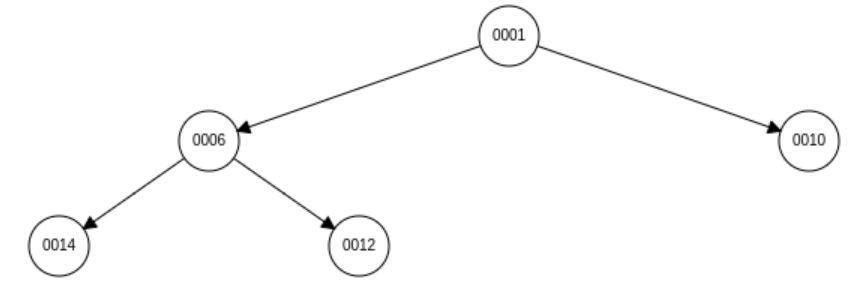
\includegraphics[width=1.04\linewidth]{hp005}
		\caption{6 se agrega como hoja pero es menor a 12, así que sube.}
		\label{fig:sfig5}
	\end{subfigure}
\begin{subfigure}{.6\textwidth}
	\centering
	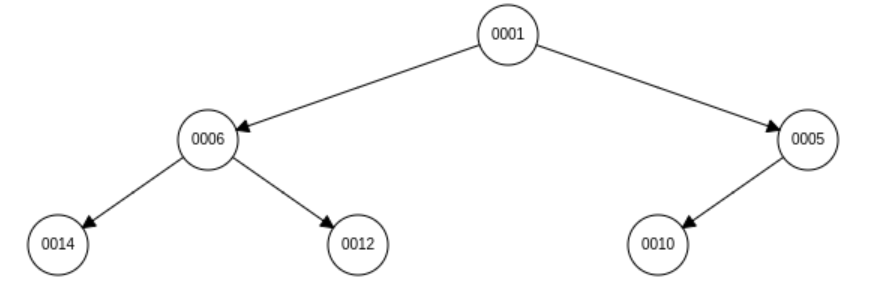
\includegraphics[width=1.04\linewidth]{hp006}
	\caption{Se agrega 5 como hoja pero es menor a 10 así que sube.}
	\label{fig:sfig6}
\end{subfigure}
\begin{subfigure}{.6\textwidth}
	\centering
	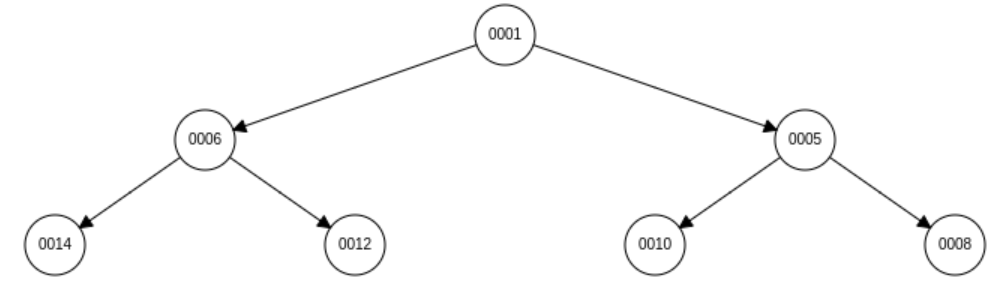
\includegraphics[width=1.04\linewidth]{hp007}
	\caption{Se agrega 8 como hoja y como es mayor a 5 se queda así.}
	\label{fig:sfig7}
\end{subfigure}
\begin{subfigure}{.6\textwidth}
	\centering
	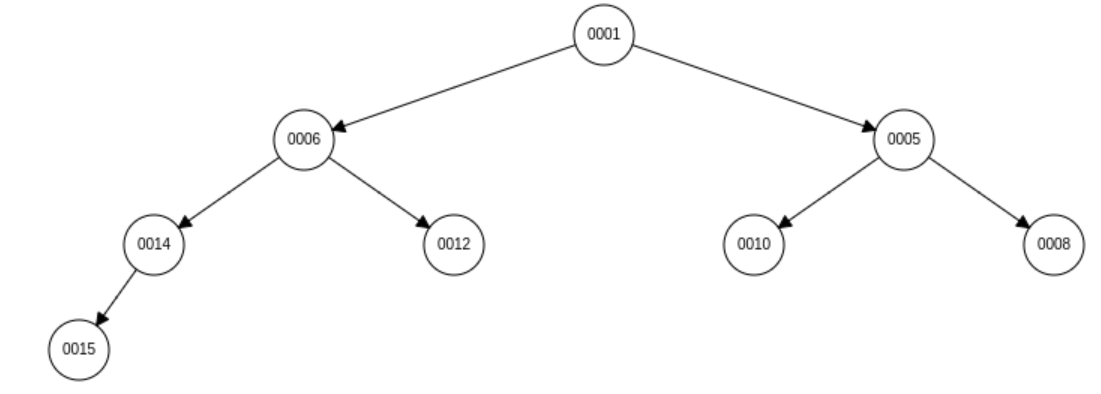
\includegraphics[width=0.95\linewidth]{hp008}
	\caption{Se agrega 15 como hoja y como es el mayor, se queda así.}
	\label{fig:sfig8}
\end{subfigure}
\begin{subfigure}{.6\textwidth}
	\centering
	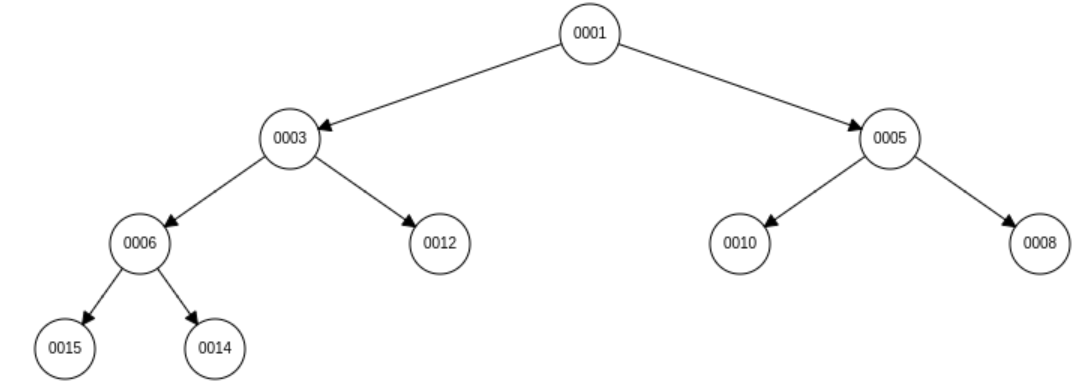
\includegraphics[width=1.04\linewidth]{hp009}
	\caption{Se agrega 3 como hoja y como es menor a 14 y a 6, sube dos niveles.}
	\label{fig:sfig9}
\end{subfigure}
	\caption{Árboles binarios en las primeras 9 inserciones.}
	\label{fig:fig}
\end{figure}
\begin{figure}
	\begin{subfigure}{.7\textwidth}
		\centering
		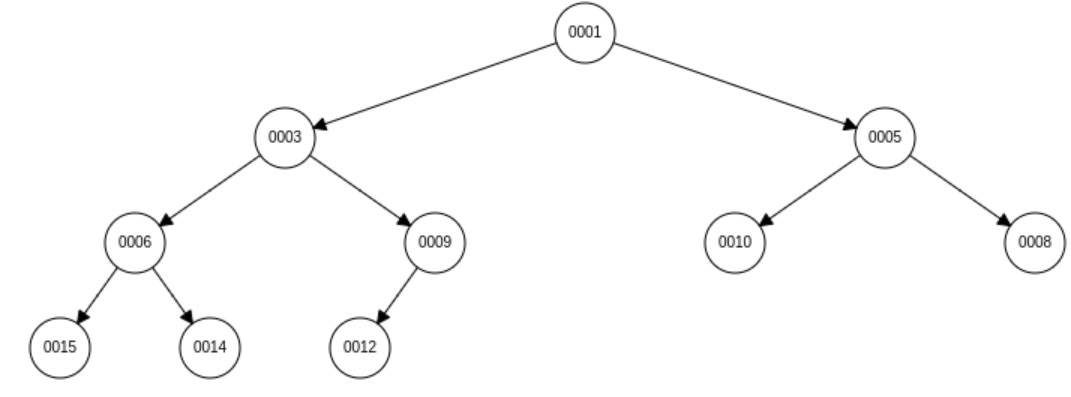
\includegraphics[width=1.1\linewidth]{hp010}
		\caption{Se agrega 9 como hoja y como es menor a 12, sube.}
		\label{fig:sfig10}
	\end{subfigure}
\begin{subfigure}{.7\textwidth}
	\centering
	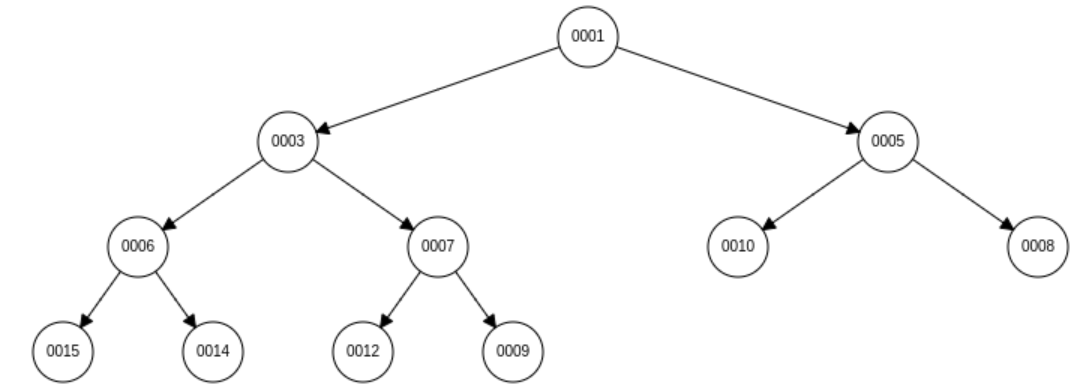
\includegraphics[width=1.1\linewidth]{hp011}
	\caption{Se agrega 7 como hoja y como es menor a 9, sube.}
	\label{fig:sfig11}
\end{subfigure}
\begin{subfigure}{.7\textwidth}
	\centering
	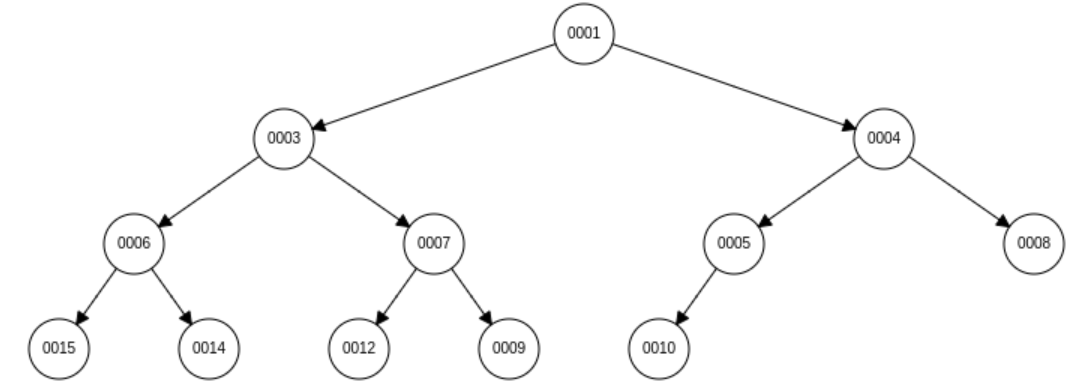
\includegraphics[width=1.1\linewidth]{hp012}
	\caption{Se agrega 4 como hoja y como es menor a 10 y 5, sube dos niveles.}
	\label{fig:sfig12}
\end{subfigure}
\begin{subfigure}{.7\textwidth}
	\centering
	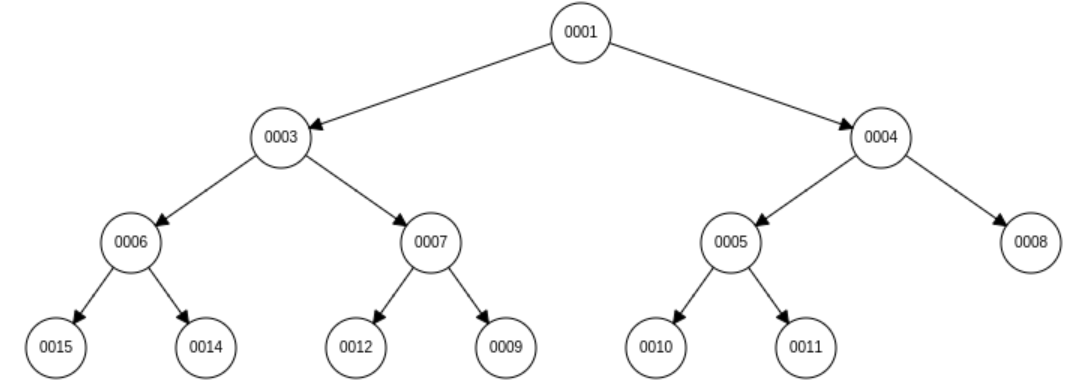
\includegraphics[width=1.1\linewidth]{hp013}
	\caption{Se agrega 11 como hoja y como es mayor a 5, se queda así}
	\label{fig:sfig13}
\end{subfigure}
	\caption{Árboles binarios en las siguientes 4 inserciones.}
	\label{fig:fig_}
\end{figure}
\begin{figure}
\begin{subfigure}{.9\textwidth}
	\centering
	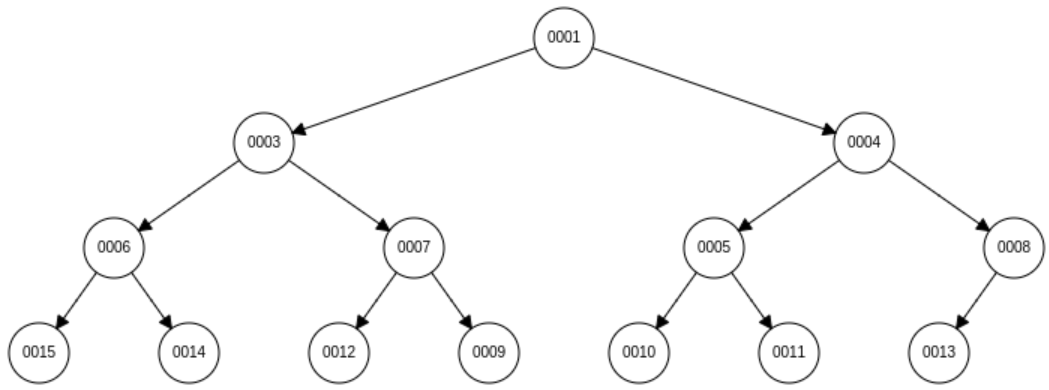
\includegraphics[width=1.2\linewidth]{hp014}
	\caption{Se agrega 13 y como es mayor a 8 así se queda. }
	\label{fig:sfig14}
\end{subfigure}
\begin{subfigure}{.9\textwidth}
	\centering
	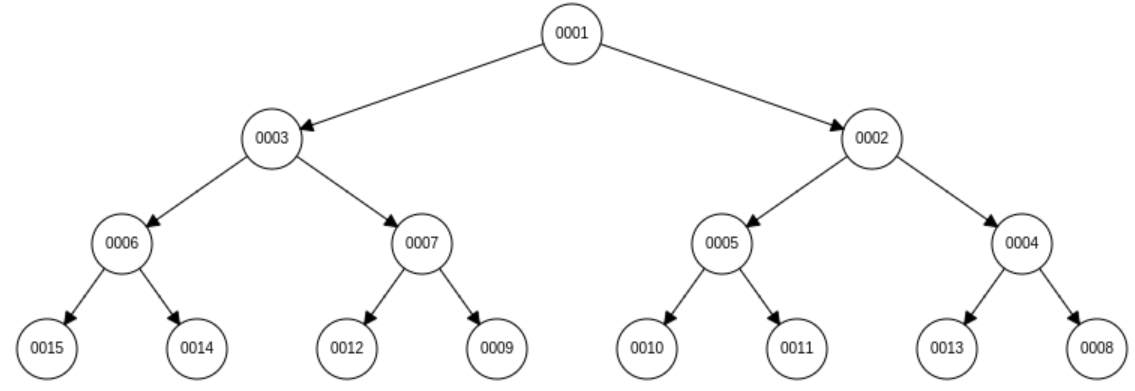
\includegraphics[width=1.2\linewidth]{hp015}
	\caption{Se agrega 2 como hoja y como es mayor a 8 y a 4, sube dos niveles.}
	\label{fig:sfig15}
\end{subfigure}
	\caption{Árboles binarios en las últimas 2 inserciones.}
	\label{fig:fig__}
\end{figure}

\end{document}